\input{configuration}

\title{Lecture 1 ---Introduction, Operating Systems, Security}

\author{Jeff Zarnett \\ \small \texttt{jzarnett@uwaterloo.ca}}
\institute{Department of Electrical and Computer Engineering \\
  University of Waterloo}
\date{\today}


\begin{document}

\begin{frame}
  \titlepage

 \end{frame}

\begin{frame}
\frametitle{Course Syllabus}

As our first order of business, let's go over the course syllabus.

\end{frame}

\begin{frame}
\frametitle{Collaborative Course}

The source material for the ECE~350 notes and slides is open-sourced via Github. 

If you find an error in the notes/slides, or have an improvement, go to \url{https://github.com/jzarnett/ece350} and open an issue. 

If you know how to use \texttt{git} and \LaTeX, then you can go to the URL and submit a pull request (changes) for me to look at and incorporate!


\end{frame}

\begin{frame}
\frametitle{Let's Talk About Labs}

Maybe we can avoid this situation?

\begin{center}
	\includegraphics[width=0.4\textwidth]{images/youridea.jpg}
\end{center}

Thanks to Prof. Zahedi for this section! 

\end{frame}

\begin{frame}
\frametitle{Lab Admin Details}

Groups are always 4 members; not 5...\\
\quad 3 requires justification.

Group split-up is possible but discouraged.

\end{frame}

\begin{frame}
\frametitle{Why Start Early?}

Estimation and planning are hard.\\
\quad New things pop up!


You don't want to be in this situation at the end of the term.
\begin{center}
	\includegraphics[width=0.75\textwidth]{images/thisisfine.jpg}
\end{center}

\end{frame}

\begin{frame}
\frametitle{Divide and Conquer}

To complete the labs effectively, work needs to be divided up.

\begin{center}
	\includegraphics[width=0.4\textwidth]{images/sandwich.jpg}
\end{center}

Overhead increases as you have more coordination.
\end{frame}

\begin{frame}
\frametitle{Dividing Work Up}

Options for how to divide it up:

\begin{itemize}
	\item Functional: by what you implement
	\item Task: Design, Implementation, Test...
	\item Time-based: Who has time to work on this right now?
	\item Maybe someone is your product (project) manager?
\end{itemize}

\end{frame}

\begin{frame}
\frametitle{Communication}

More people means more communication and more overhead.

Err on the side of over-communication!\\
\quad Otherwise misunderstandings are possible: index starts at 0 or 1?

Write decisions and important information down!

\end{frame}

\begin{frame}
\frametitle{Decision-Making}

Individual decisions are fast, but group decisions may be best.

\begin{center}
	\includegraphics[width=0.65\textwidth]{images/proverb.jpeg}
\end{center}

Let those who know the most about the problem/area have the final call!

Is someone your system architect? Big picture view.

\end{frame}

\begin{frame}
\frametitle{What's Done is Done}

Did I mention you should write down decisions? 
\begin{center}
	\includegraphics[width=0.4\textwidth]{images/writedown.jpg}
\end{center}

When a decision is made, even if you disagree, go with it.

\end{frame}

\begin{frame}
\frametitle{Work Styles}

It's important that you choose group members with compatible work styles.

When I am consultant for a capstone group I ask if they agree on:

\begin{itemize}
	\item Ahead-of-the-game or last-minute?
	\item Have you worked together before?
	\item How far do you want to take this?
\end{itemize}

\end{frame}

\begin{frame}
\frametitle{How to Make It Work}
Some general advice:

\begin{itemize}
	\item Communication is key; write stuff down.
	\item Planning is valuable even if things don't go to plan
	\item Don't stay mad if someone makes a mistake or misses a meeting
	\item Put ego to the side
	\item Use good coding practices: git, automated tests, code review, etc.
\end{itemize}

\end{frame}

\begin{frame}
\frametitle{Test Early, Test Often}

Test all along the way, not just at the end.

Unit tests and integration tests.

Also try messing with the timing to ensure it doesn't break things!

\end{frame}

\begin{frame}
\frametitle{It's Hard}

The labs are not easy, but they are a very valuable learning experience.

\begin{center}
	\includegraphics[width=\textwidth]{images/worthit.jpg}
\end{center}

\end{frame}

\begin{frame}
\frametitle{Introduction to Operating Systems}

\begin{quote}
\textit{Operating systems are those programs that interface the machine with the applications programs. The main function of these systems is to dynamically allocate the shared system resources to the executing programs.}
\end{quote}

\hfill - What Can Be Automated?: The Computer Science and Engineering Research Study, MIT Press, 1980

\end{frame}


\begin{frame}
\frametitle{Introduction to Operating Systems}

\begin{center}
	\includegraphics[width=.6\textwidth]{images/linux-user.jpg}
\end{center}


\end{frame}


\begin{frame}
\frametitle{Introduction to Operating Systems}

An operating system (OS) sits between the hardware and programs.

It has many goals, that often conflict with one another.

Its job is to make it so other programs can run efficiently.

\end{frame}

\begin{frame}
\frametitle{Structural Diagram of a Modern Computer}

\begin{center}
\includegraphics[width=0.95\textwidth]{images/os-sw-hw.png}
\end{center}

\end{frame}


\begin{frame}
\frametitle{OS: Resource Manager}

The OS is responsible for resource management and allocation.

Resources like CPU time or memory space are limited.

The OS must decide how to allocate \& to keep track of system resources.

In the event of conflicting requests, choose the winner.


\end{frame}

\begin{frame}
\frametitle{OS: Environment Provider}

The OS enables useful programs like Photoshop or Microsoft Word to run. 

The OS is responsible for abstracting away the details of hardware.

This is so program authors do not have to worry about the specifics.

Imagine Hello World had to be written differently for different hardware.


\end{frame}

\begin{frame}
\frametitle{OS: Multitasking}
Multiple programs means some resources are shared.\\
\quad $\rightarrow$ A source of conflicts!

OS creates and enforces the rules so all can get along.

\begin{center}
	\includegraphics[width=0.4\textwidth]{images/sharing-is-caring.jpg}
\end{center}

Sometimes processes want to co-operate and not compete.\\
\quad The OS can help them to do so.


\end{frame}

\begin{frame}
\frametitle{OS: Efficiency}
Another goal may be to use the computer hardware efficiently.

\begin{center}
	\includegraphics[width=0.7\textwidth]{images/supercomputer.jpg}
\end{center}
\hfill Image Credit: Argonne National Laboratory

Any moment when the supercomputer is not doing useful work is a waste.

\end{frame}

\begin{frame}
\frametitle{OS: What is it, really?}

Operating systems tend to be large and do a lot of things. 

We expect now that an OS comes with a web browser, an e-mail client, some method for editing text, et cetera. 

The part of the operating system we will study is the \alert{Kernel}.

The kernel is the ``core''; the portion of the OS that is always present in main memory and the central part that makes it all work.

\end{frame}

\begin{frame}
\frametitle{OS: Evolution}
Operating systems will evolve over time. 

There will be new hardware released, new types of hardware, new services added, and bug fixes. 

Evolution is constrained: a need to maintain compatibility for programs. 

\begin{center}
	\includegraphics[width=0.7\textwidth]{images/linus-angry.jpg}
\end{center}

\end{frame}


\begin{frame}
\frametitle{Example: SimCity and Windows 95}

\begin{center}
	\includegraphics[width=0.85\textwidth]{images/simcity.png}
\end{center}

\end{frame}


\begin{frame}
\frametitle{Time, What is Time?}

\begin{center}
	\includegraphics[width=0.4\textwidth]{images/10thdoctor.jpg}
\end{center}

\textit{People assume that time is a strict progression from cause to effect, but actually from a non-linear, non-subjective viewpoint, it's more like a big ball of wibbly-wobbly, timey-wimey stuff.}


\end{frame}



\begin{frame}
\frametitle{Real-Time vs. Non Real-Time}

Real-time systems are the ones where wall-clock deadlines matter.

Examples: aviation, industrial machinery, video conferencing, satellites...

\end{frame}

\begin{frame}
\frametitle{Real-Time Scheduling}

There are deadlines, and there are consequences for missing deadlines. 

\begin{center}
	\includegraphics[width=\textwidth]{images/ticktock.jpg}
\end{center}

Fast is not as important as predictable.

\end{frame}

\begin{frame}
\frametitle{Hard and Soft Real-Time}

\alert{Hard real-time}: it has a deadline that must be met to prevent an error, prevent some damage to the system, or for the answer to make sense. 

If a task is attempting to calculate the position of an incoming missile, a late answer is no good. 

A \alert{soft real-time} task has a deadline that is not, strictly speaking, mandatory; missing the deadline degrades the quality of the response, but it is not useless.


\end{frame}



\begin{frame}
\frametitle{Security Now}

\begin{center}
	\includegraphics[width=0.9\textwidth]{images/security-team.png}
\end{center}


\end{frame}


\begin{frame}
\frametitle{Security Now}

In many textbooks, security and protection are left to the end.

Security has to be designed from the beginning; cannot be bolted on.

An OS supports multiple users with multiple tasks.

\end{frame}


\begin{frame}
\frametitle{Tool Support}

OS designers create policies and policy tools.

There is a tradeoff with usability.

You do NOT want to have to report a data breach.

\begin{center}
	\includegraphics[width=0.35\textwidth]{images/security-budget.png}
\end{center}


\end{frame}


\begin{frame}
\frametitle{Enforcement is Everything}

The OS must enforce the configured policies.\\
\quad Otherwise, malicious users exploit it.

Three desirable properties: Confidentiality, Integrity, Availability.

\end{frame}


\begin{frame}
\frametitle{Protection vs Security}

Protection is about internal threats.

Security is about external threats.

We'll take them in order.


\end{frame}


\begin{frame}
\frametitle{Protection}

\begin{center}
	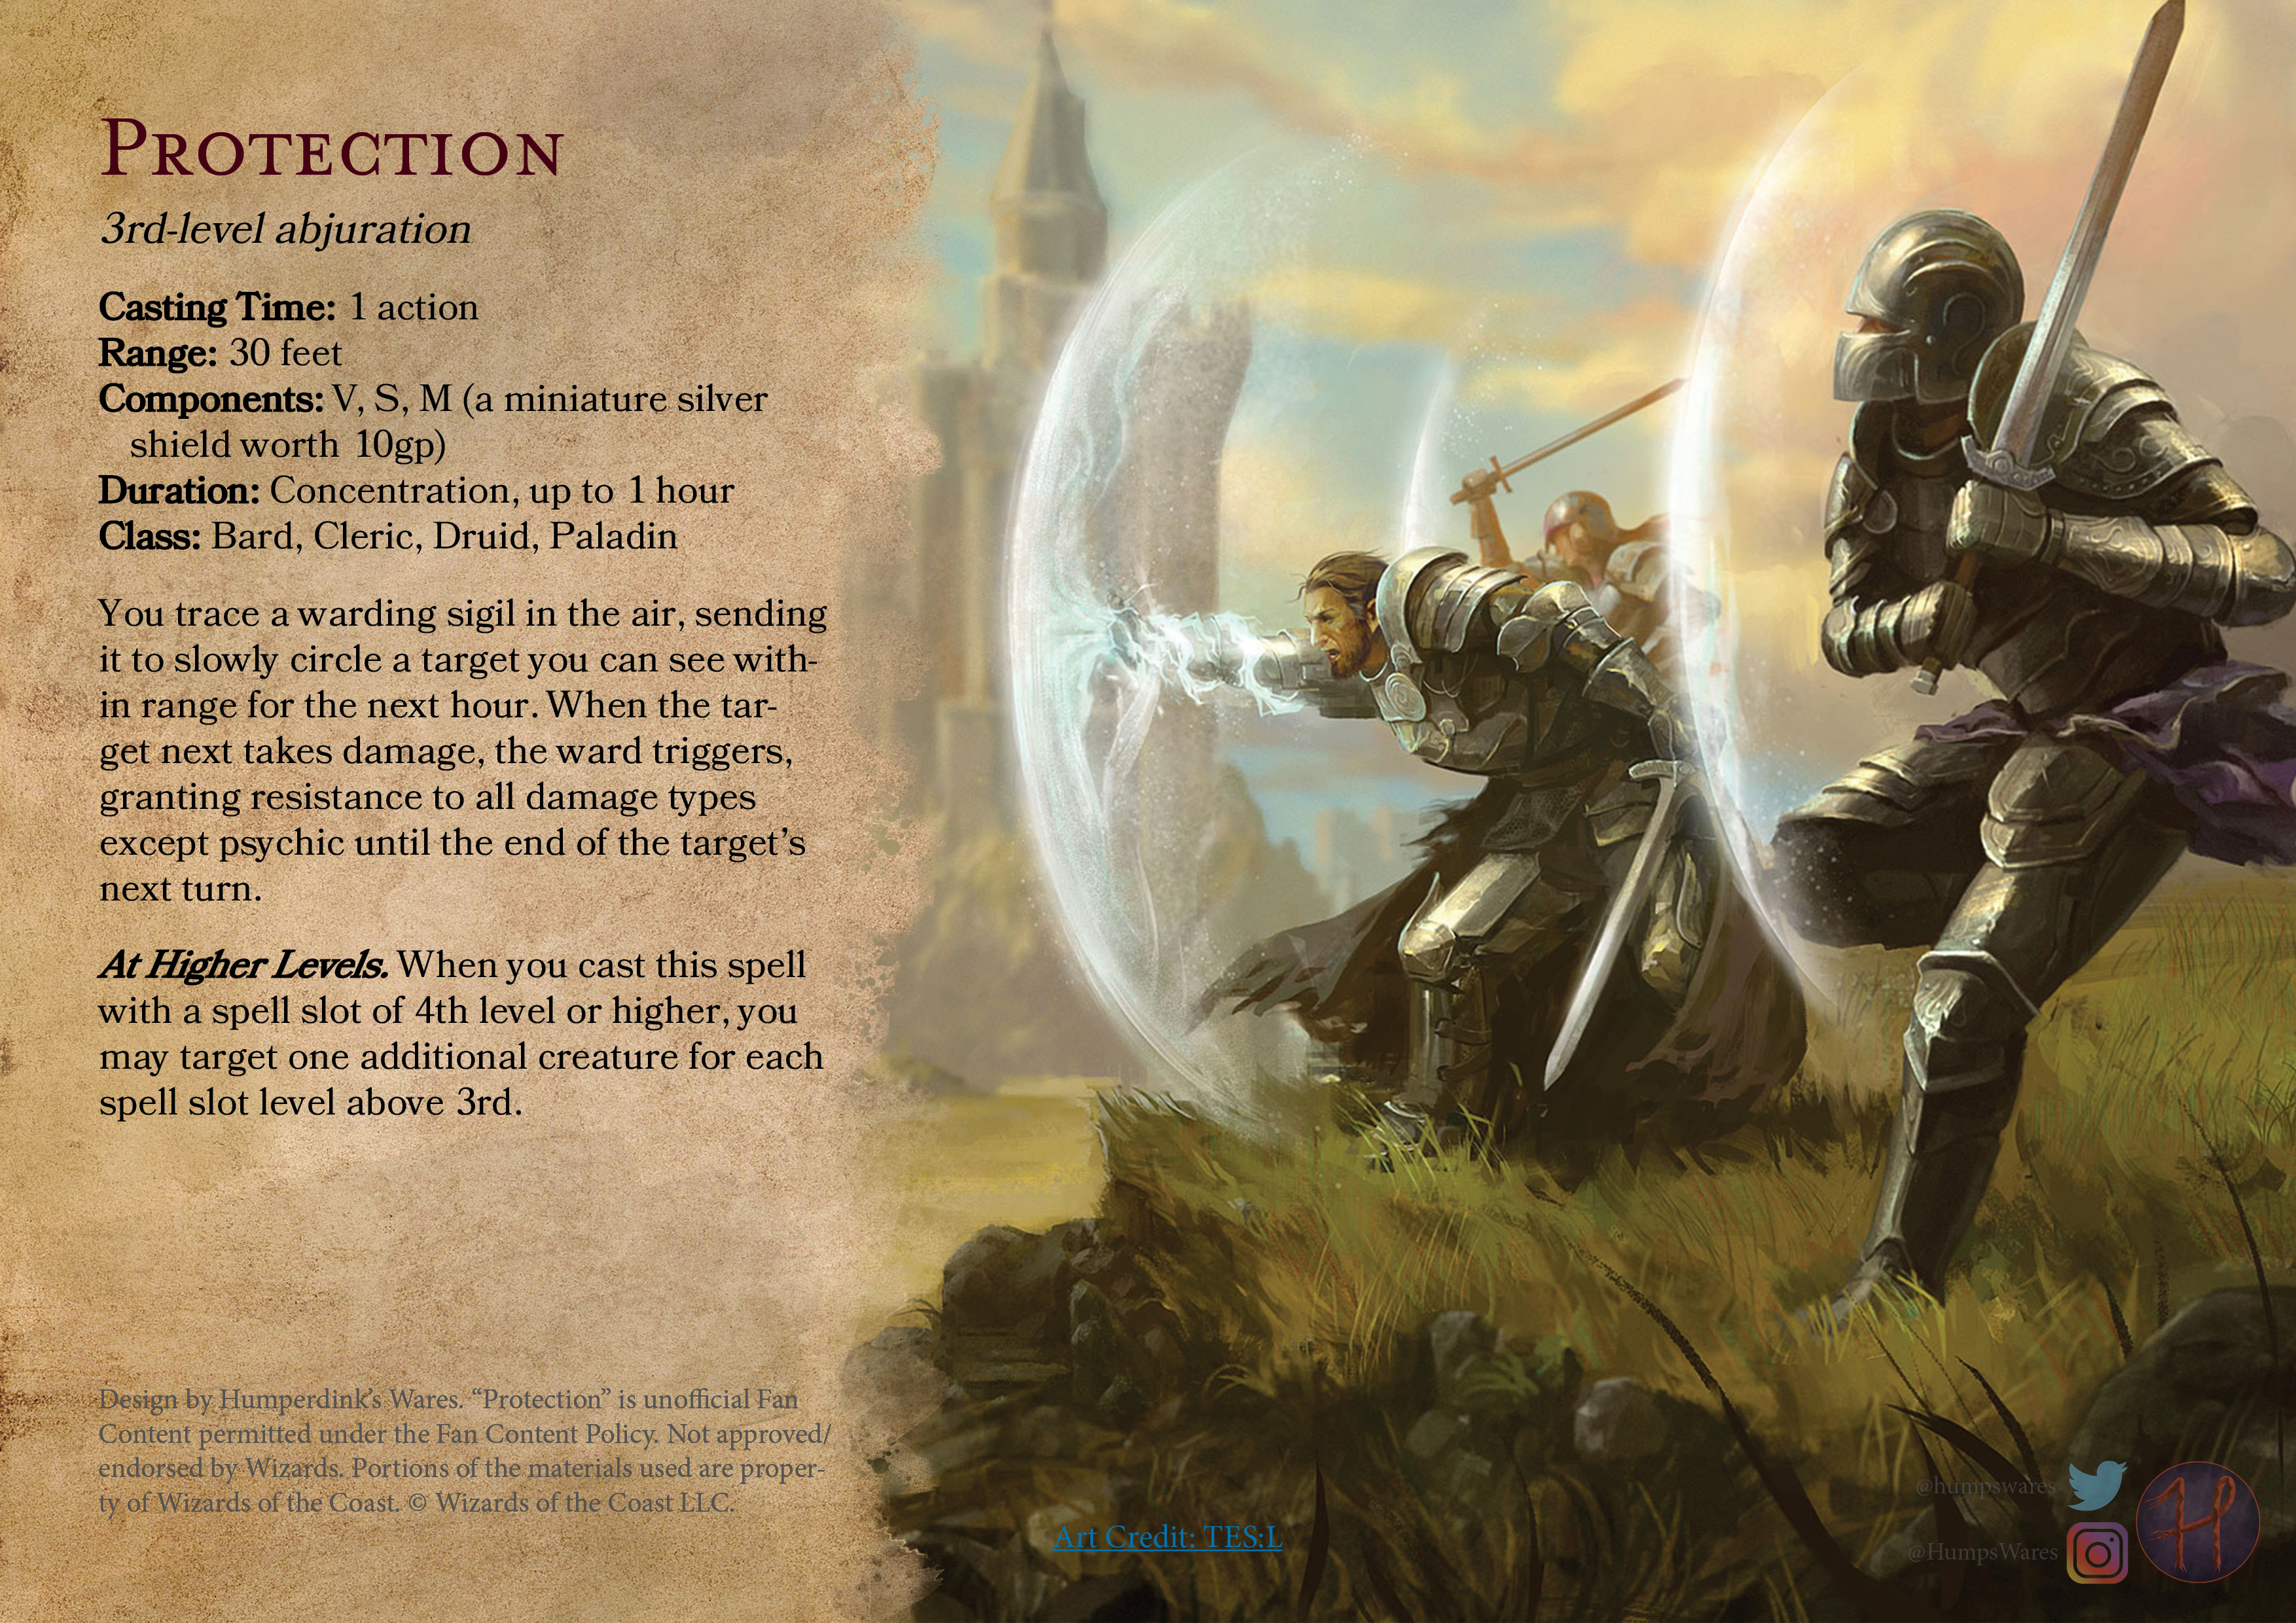
\includegraphics[width=\textwidth]{images/protection.jpg}
\end{center}


\end{frame}

\begin{frame}
\frametitle{Protection}

Most of the discussion in this course is about protection.

Following the rules is important to a functioning system or society.

Even in the absence of malicious intent.


\end{frame}


\begin{frame}
\frametitle{Goals of Protection}

Enforce policies about responsible usage.

Responsible and reasonable vary across systems.

Examples of access control: file permissions, walls between processes.

\end{frame}


\begin{frame}
\frametitle{Enforcement is Key}

Rules take effort to enforce.

Exceptions are allowed and administrators can override policies!

\begin{center}
	\includegraphics[width=0.4\textwidth]{images/override.jpg}
\end{center}

Other kinds of rules can exist.

\end{frame}


\begin{frame}
\frametitle{Context is Key}

If I edit a lecture video, it consumes a lot of CPU and RAM.

Is that bad?

It's legitimate -- but might set off alarms.

So we may be lax -- which gives an opening to malicious users...


\end{frame}



\begin{frame}
\frametitle{Security}

\begin{center}
	\includegraphics[width=0.4\textwidth]{images/security-alert.png}
\end{center}

Let's consider a few bad things attackers can do.

Why? We need this in mind when designing the system.


\end{frame}


\begin{frame}
\frametitle{Security Problems}

\begin{itemize}
	\item Breach of Confidentiality
	\item Breach of Integrity
	\item Breach of Availability
	\item Theft of Service
	\item ... and others.
\end{itemize}

Most likely the weak link is people.

\end{frame}


\begin{frame}
\frametitle{Specific Attacks}
A few potential specific attacks:

\begin{itemize}
	\item \textbf{Excessive Requests}
	\item \textbf{Malformed Requests}
	\item \textbf{Back Door}
	\item \textbf{Intercepting Messages}
	\item \textbf{Trojan Horse}
\end{itemize}


\end{frame}


\begin{frame}
\frametitle{Arms Race}

Security is an arms race.

Can we break things if it's a security problem?

No easy answers.


\end{frame}


\begin{frame}
\frametitle{Security, Conclusion}

This is not a course in security, but we can't ignore it.

Security needs to be included from the beginning!


\end{frame}

\begin{frame}
\frametitle{ONE MORE ROUND!}

Remember when Ivan Drago said ``I must break you''? 

\begin{center}
	\includegraphics[width=0.5\textwidth]{images/one-more-round.jpg}
\end{center}
\hfill \textit{``I didn't hear no bell. One more round!''} -- Rocky Balboa

This course is challenging too, but in a different way.\\
\quad There are a lot of topics and we have to move fast.\\
\quad And the labs can consume a lot of time.

\end{frame}


\begin{frame}
\frametitle{The Plan}

A broad overview of the major topics of the course:

\begin{enumerate}
	\item Introduction, Security, Review from ECE 252
	\item Memory
	\item Scheduling
	\item I/O Devices, File Systems
	\item Reliability, Virtualization/Containers
\end{enumerate}

\end{frame}



\end{document}

